\documentclass[11pt,a4paper]{article}
\usepackage[utf8]{inputenc}
\usepackage[T1]{fontenc}
\usepackage{geometry}
\geometry{margin=2.5cm,headheight=14pt}
\usepackage{longtable}
\usepackage{booktabs}
\usepackage{array}
\usepackage{colortbl}
\usepackage{xcolor}
\usepackage{graphicx}
\usepackage{hyperref}
\usepackage{enumitem}
\usepackage{titlesec}
\usepackage{fancyhdr}
\usepackage{tabularx}
\usepackage{multirow}
\usepackage{amsmath}
\usepackage{float}
\usepackage{tikz}
\usepackage{pgfplots}
\pgfplotsset{compat=1.17}
\usepackage{pgf-pie}

\definecolor{uteqblue}{RGB}{11,61,109}

\hypersetup{colorlinks=true, linkcolor=blue, citecolor=blue, urlcolor=blue}

\pagestyle{fancy}
\fancyhf{}
\fancyhead[L]{UTEQ -- Ingeniería de Requisitos [ISR-401]}
\fancyhead[R]{PE4 -- Unidad IV -- CarniCore}
\fancyfoot[C]{\thepage}

\newcommand{\logoplaceholder}{%
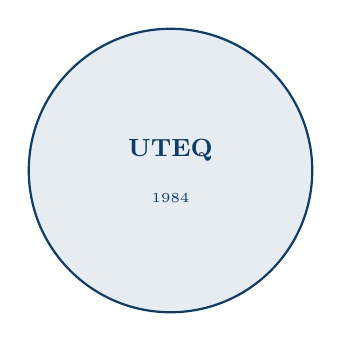
\begin{tikzpicture}
\draw[uteqblue, thick, fill=uteqblue!10] (0,0) circle (1.8cm);
\node[uteqblue, font=\bfseries\small, align=center] at (0,0.25) {UTEQ};
\node[uteqblue, font=\tiny, align=center] at (0,-0.35) {1984};
\end{tikzpicture}%
}

\title{
\vspace{-1.5cm}
\textbf{Práctica Experimental -- Unidad IV}\\[0.2cm]
\Large Validación, Gestión de Requisitos y Herramientas CASE\\[0.15cm]
\large Inspección Fagan \(\cdot\) CCB \(\cdot\) Trazabilidad CASE \(\cdot\) Baseline Git\\[0.35cm]
\normalsize Asignatura: Ingeniería de Requisitos [ISR-401]\\
Período: 2026--2027 PPA\\
Unidad: IV -- Semana 14\\
Sistema PFC: CarniCore -- Sistema de Trazabilidad, Pesaje Inteligente e Inventario\\
para Distribuidora de Cárnicos Pucayacu -- La Maná, Cotopaxi
}
\author{Universidad Técnica Estatal de Quevedo (UTEQ)\\Facultad de Ciencias de la Computación y Diseño Digital\\Carrera de Software (Rediseño)}
\date{Quevedo, Ecuador -- 4 de agosto de 2026}

\begin{document}

\title{Documento Evidencia — MDD}
\author{}
\date{}


\begin{titlepage}
\centering

\textbf{\large UNIVERSIDAD TÉCNICA ESTATAL DE QUEVEDO}\\[0cm]


\includegraphics[width=5cm]{figuras/logo.png}

\textbf{PRÁCTICA EXPERIMENTAL – UNIDAD IV}\\[0.8cm]

\textbf{TEMA:}\\[0.4cm]

Validación, Gestión de Requisitos y Herramientas CASE
Inspección Fagan · CCB · Trazabilidad CASE · Baseline Git.\\[0.8cm]

\textbf{INTEGRANTES:}\\[0.5cm]

AMAGUA SACON ROBYN WILLIAN\\[0.5cm]
CRESPO ESPINOZA KLEBER OBED\\[0.5cm]
GAMARRA ARAUJO EDHU XAVIER\\[0.5cm]
PONCE ESPINOZA MERY HELENMAY\\[0.8cm]

\textbf{ASIGNATURA:}\\[0.5cm]

INGENIERÍA DE REQUERIMIENTOS\\[0.5cm]

\textbf{CURSO:}\\[0.2cm]

4TO ``A'' SOFTWARE\\[0.5cm]

\textbf{FECHA:}\\[0.2cm]

04/08/2026\\[0.8cm]

\textbf{DOCENTE:}\\[0.2cm]

ING. GUERRERO ULLOA GLEISTON CICERON\\[0.5cm]

\textbf{LINK DE GITHUB:}\\[0.2cm]

\url{https://github.com/EdhuXav/EdhuXav-ISR401-PFC-ERS-EquipoJ}

\vspace*{1cm}

Último commit 5 de agosto a las 23:00 horas
\end{titlepage}


\newpage
\tableofcontents
\newpage

%======================================================
\section{Resumen y Objetivos}
%======================================================
\subsection{Resumen}
La presente práctica experimental aplica técnicas formales de validación de requisitos,
gestión del cambio y trazabilidad sobre la Especificación de Requisitos Software (ERS)
del sistema \textbf{CarniCore} -- Sistema de Trazabilidad, Pesaje Inteligente e Inventario para la
Distribuidora de Cárnicos Pucayacu (La Maná, Cotopaxi) --, proyecto fin de curso del equipo.
Se ejecutó una inspección formal Fagan con cinco roles diferenciados sobre las secciones 1 a 3
del ERS v3.0 (25 RF y 15 RNF), se registraron y corrigieron los defectos hallados, y se tramitaron
tres solicitudes de cambio (RFC) ante un Change Control Board (CCB) simulado. Posteriormente,
la trazabilidad bidireccional del ERS se implementó en Jira, se estableció la línea base mediante
control de versiones Git con etiqueta anotada y CHANGELOG, y se compararon metodológicamente
herramientas CASE de IR y enfoques tradicional versus ágil. El informe cierra con cinco
conclusiones críticas derivadas de los artefactos propios del equipo.

\subsection{Objetivo General}
Aplicar técnicas formales de validación de requisitos, gestionar cambios mediante un
CCB simulado, implementar la trazabilidad del ERS en una herramienta CASE, establecer
una línea base con Git y comparar metodológicamente la IR tradicional frente a la IR
ágil, sobre el ERS real del sistema CarniCore.

\subsection{Objetivos Específicos}
\begin{enumerate}[nosep]
\item Ejecutar una inspección formal tipo Fagan sobre el ERS de CarniCore con roles diferenciados, lista de verificación y registro de defectos.
\item Calcular e interpretar métricas de inspección (densidad de defectos, distribución por tipo y severidad, tasa de corrección).
\item Tramitar tres RFC con análisis de impacto sustentado en la matriz de trazabilidad.
\item Deliberar y decidir en un CCB simulado, dejando acta motivada y versión actualizada del ERS.
\item Construir la trazabilidad bidireccional del ERS en Jira con campos personalizados y enlaces verificables.
\item Establecer y publicar la línea base del ERS con commit semántico, tag anotado y CHANGELOG.md.
\item Comparar herramientas CASE de IR y contrastar IR tradicional frente a IR ágil con conclusiones críticas propias.
\end{enumerate}


\end{document}
